\documentclass{beamer}
 % \usetheme{metropolis}
% \usetheme{confposter}
\usepackage[orientation=portrait, size=a0, scale=1]{beamerposter}
% \usepackage[scale=1.7,size=a1]{beamerposter}
\setlength{\paperwidth}{33.1in}
\setlength{\paperheight}{23.4in}
\usepackage[utf8]{inputenc}
\usepackage[english]{babel}
\usepackage[T1]{fontenc}
\usepackage{lmodern}
\usepackage{exscale}
\usepackage{amsmath}
\usepackage{amsfonts}                                                                               
\usepackage{amssymb}
\usepackage{bm}
\usepackage{wrapfig}
\usepackage{bbm}
\usepackage{subfig}
\usepackage{fix-cm}    
\usepackage{multicol}
\usepackage{pgfplots}       
\usepackage[absolute,overlay]{textpos}

\definecolor{blkcol}{HTML}{E1E1EA}
\definecolor{blkcol2}{RGB}{209, 224, 224}
\definecolor{palered}{HTML}{FFD8D8}
\definecolor{darkprimcol}{HTML}{455A64}
\definecolor{lightprimcol}{HTML}{CFD8DC}
\definecolor{primcol}{HTML}{607D8B}
\definecolor{accentcol}{HTML}{448AFF}
\definecolor{primarytxt}{HTML}{212121}
\definecolor{secondtxt}{HTML}{757575}
\definecolor{dividertxt}{HTML}{BDBDBD}
\definecolor{bll}{HTML}{355C7D}
\definecolor{mist}{HTML}{90AFC5}
\definecolor{autumn}{HTML}{763626}

% \setbeamercolor{block title}{bg = blkcol}
\setbeamercolor{block body}{bg = mist!10}
\setbeamercolor{block body alerted}{bg = palered!50}
\setbeamercolor{block title}{bg = bll, fg = white}
% \setbeamercolor{block body}{bg = lightprimcol}
% \setbeamercolor{block body alerted}{bg = accentcol!50}
\setbeamercolor{bibliography item}{fg=bll}
\setbeamercolor*{bibliography entry title}{fg=bll}
\setbeamercolor*{bibliography entry author}{fg=bll}
\setbeamercolor*{bibliography entry location}{fg=bll}
\setbeamercolor*{bibliography entry note}{fg=bll}

\addtobeamertemplate{block begin}{\vskip + 0.2\smallskipamount}{} 
\addtobeamertemplate{block end}{}{\vskip + 0.2\bigskipamount}
\setbeamerfont{itemize/enumerate body}{}
\setbeamerfont{itemize/enumerate subbody}{size=\normalsize}
\setbeamerfont{itemize/enumerate subsubbody}{size=\footnotesize}
\graphicspath{{./Figures/}}

\makeatletter
\newcommand\HUGE{\@setfontsize\Huge{83}{90}}
\makeatother    
%----------------------------------
\newlength{\sepwid}
\newlength{\onecolwid}
\newlength{\twocolwid}
\newlength{\threecolwid}
\newlength{\thirdcolwid}
\newlength{\sndcolwid}
\newlength{\leftmar}
\newlength{\centercol}
\setlength{\paperwidth}{36in} % A0 width: 46.8in
\setlength{\paperheight}{48in} % A0 height: 33.1in
\setlength{\leftmar}{0.035 \paperwidth}
% \setlength{\sepwid}{0.005 \paperwidth} % Separation width (white space) between columns
\setlength{\sepwid}{0.012 \paperwidth} % Separation width (white space) between columns

\setlength{\onecolwid}{0.22\paperwidth} % Width of one column
\setlength{\twocolwid}{0.464\paperwidth} % Width of two columns
\setlength{\threecolwid}{0.708\paperwidth} % Width of three columns
\setlength{\topmargin}{-.4in} % Reduce the top margin size
\setlength{\thirdcolwid}{.301\paperwidth}
\setlength{\sndcolwid}{.4555\paperwidth}
\setlength{\centercol}{0.93\paperwidth}
%------------------------------------
\newcommand{\Ex}{\mathbb{E}}
\newcommand{\Var}{\mathbb{V}\mathrm{ar}}
\newcommand{\Prob}{\mathbb{P}}
\DeclareMathOperator*{\argmin}{arg\,min}
\DeclareMathOperator*{\argmax}{arg\,max}
\newcommand{\Cov}{\textsf{Cov}}

\newcommand{\tra}{\mathrm{tr}}
\newcommand{\yobs}{\bm{y}_{\mathrm{obs}}}
\newcommand{\kest}{\hat{\bm{k}}}
\DeclareMathOperator*{\KL}{\textsf{KL}}


\setbeamertemplate{headline}{
 \leavevmode
  \begin{columns}
   % \begin{column}{.01\linewidth}
   % \end{column}
    \hspace{-1in}
   \begin{column}{.80\linewidth}
     \vskip0.5cm
     \begin{center}
      \usebeamercolor{title in headline}{\color{fg}{\HUGE \inserttitle} \\[2ex]}
    \usebeamercolor{author in headline}{\color{fg}{\huge \insertauthor }\\[1ex]}
    \usebeamercolor{institute in headline}{\color{fg}\large{\insertinstitute}\\[0.1ex]}
  \end{center}

    % \vskip0.5cm
   \end{column}
   \begin{column}{.15\linewidth}
     
\includegraphics{INRIA_SCIENTIFIQUE_UK_CMJN} \\
     
\includegraphics{ljk}
   \end{column}
   \vspace{1cm}
 \end{columns}
 \vspace{0.2in}
 \hspace{0.5in}\begin{beamercolorbox}[wd=47in,colsep=0.15cm]{cboxb}\end{beamercolorbox}
 \vspace{-0.2in}  
}

\title{Parameter control in the presence of uncertainties} 
\author{Victor Trappler \\{\Large \texttt{victor.trappler@univ-grenoble-alpes.fr}}\\ {\LARGE Élise Arnaud, Laurent Debreu, Arthur Vidard} }
\institute{\large AIRSEA Research team (Inria) -- Laboratoire Jean Kuntzmann \\[2ex]
\textsc{Workshop on Sensitivity Analysis and Data Assimilation in
  Meteorology and Oceanography, Aveiro, Portugal 2018}}
% \textsc{$7^{\mathrm{th}}$ PHD Day, ED MSTII, Grenoble 2018} }
% \titlegraphic{
\includegraphics[scale=2]{INRIA_SCIENTIFIQUE_UK_CMJN}
% 
\includegraphics[scale=1]{ljk}}


\date{}

\listfiles
\begin{document}
\begin{frame}[t]
% \maketitle
% \noindent\rule{\paperwidth}{1.5pt}
  \begin{columns}[t]
    \begin{column}{\leftmar}\end{column}
    \begin{column}{\centercol}

      
            {\Large How can one calibrate a numerical model so that it performs reasonably well for different random operating conditions ?
}
     \large       
    \begin{alertblock}{Objectives}
      % Complex subgrid phenomena have to be parametrized in numerical models, and those values have to be properly estimated. This task is further complicated by the presence of uncertainties modelled by random variable. The calibrated value of the parameter is directly dependent on uncertainties.

      % Strategies taking into account those uncertainties are to be defined and applied on an academic model of a coastal area, in order to find an optimal value in a robust sense. 
    \begin{itemize}
    \item Define suitable \alert{definitions of robustness} in the field of computer code calibration
    \item Develop \alert{efficient} techniques and algorithms in order to estimate those parameters
    \item Deal with the high-dimension of the parameter spaces: \alert{Dimension reduction }
    \end{itemize}
  \end{alertblock}
\end{column}
\end{columns}
\vspace{0.2in}
\begin{columns}[t] % The whole poster consists of three major columns, the second of which is split into two columns twice - the [t] option aligns each column's content to the top

\begin{column}{\leftmar}\end{column} % Empty spacer column

\begin{column}{\sndcolwid} % The first column

  \begin{block}{Background: estimation of the bottom friction in a shallow water model}
    % {\large Computer model: 2 inputs}
    %  \begin{itemize} 
    % \item $\bm{k}\in\mathcal{K}$: the control/decision parameter
    % \item $\bm{u}\in\mathcal{U}$: the uncertain variable representing the environmental conditions
    % \end{itemize}  
    \begin{figure}[!h]
      \centering
      \resizebox{.7\linewidth}{0.05\textheight}{\begin{tikzpicture}
\usetikzlibrary{decorations.pathmorphing}

\definecolor{copper}{rgb}{0.69, 0.25, 0.21}
\definecolor{tin}{rgb}{0.7, 0.7, 0.7}

\tikzset{
  rugous1/.style = {black, thick,
    decoration={random steps,segment length=0.05cm,amplitude=.1cm}
  },
}
\tikzset{
  rugous2/.style = {black, thick,
    decoration={random steps,segment length=0.2cm,amplitude=.05cm}
  },
}
\tikzset{
  rugous3/.style = {black, thick,
    decoration={random steps,segment length=0.2cm,amplitude=.15cm}
  },
}

\filldraw [fill = blue!30]
   plot [samples = 100,domain = -5:5] (\x, {0.5*sin(\x r) + 2} )
-- plot [samples = 100,domain = 5:-5] (\x, {0.3*sin(\x/1.5 r)+0.5})
-- cycle;

\filldraw[fill = gray!30, draw = white]
   plot [samples = 100,domain = -5:5] (\x, {0.3*sin(\x/1.5 r)+0.5})
-- plot [samples = 100,domain = 5:-5] (\x, 0)
-- cycle;

\draw[rugous1, decorate](-5,0.52) -- (-2.3,0.2);
\draw[rugous2, decorate](-2.3,0.2) -- (2.4,0.8);
\draw[rugous3, decorate](2.4,0.8) -- (5,0.5);

\draw[->] (-5,0) -- (5,0);
\draw (0,0) node[below] {$x$};



\draw[->] (-5,0) -- (-5,3);

\draw[->] (0,0.5) -- (0,2);
\draw (0, 1.25) node[left] {$h(x,t)$} ;
\draw (0,0) node[below] {$x$};
\draw[->] (2,0) -- (2,{0.3*sin(2/1.5 r)+0.5});
\draw (2, 0.3) node[right] {$Z(x)$} ;
\draw[->] (1,0) -- (1,{0.5*sin(1 r)+2});
\draw (1, 1.3) node[right] {$H(x,t)$} ;
\end{tikzpicture}}
    \end{figure}
    The calibration problem is to be able to find a value of $\bm{k}\in\mathcal{K}$ denoted $\kest$ that matches the best the observations $\yobs$  \nocite{bayarri_framework_2007}
. We define a loss function, that is the misfit between the observations to the model. 

    
% \usetikzlibrary{positioning}
\tikzstyle{block} = [rectangle, draw, fill=blue!30, 
    text centered, minimum width=10em] 
%  \tikzstyle{block} = [rectangle, draw, fill=blkcol, 
%       text centered, minimum width=3em]

% \tikzstyle{block2} = [rectangle, draw, fill=blkcol2, 
%      text centered, rounded corners, minimum width=3em]
% 
% \tikzstyle{block2} = [rectangle, draw, fill=blkcol2, 
%      text centered, rounded corners, minimum width=3em]

\tikzstyle{LHS}=[rectangle, draw, text centered]
\begin{center}
\begin{tikzpicture}[node distance= 2em]

%\node [align = center] at (0,0) (input) {Control variable \\$\bm{k} \in \mathcal{K}$};
\node [align = center]  (input) {Control variable \\$\bm{k} \in \mathcal{K}$};
\node[block ,right =  of input](code){Direct Simulation};
%\node [align = center, above =of  code ] (envir) {Environmental variables \\$\mathbf{u} \in \mathcal{U}$ fixed};
\node [align = center, above = of code] (envir) {Environmental variables \\$\bm{u} \in \mathcal{U}$ fixed};





\node[align = center, right = of code]  (output) {$M(\bm{k})$}; 
\node[block, below =of code] (inv) {Inverse Problem};
\node [align = center, right = of inv,  below =  of output] (obs) {$\yobs$};

\draw[->] (input) -- (code);
\draw[->] (envir) -- (code);
\draw[->] (code) -- (output);

 % \node [align = center] at (0,0) (input) {$Y = \mathcal{H}W(K_{\mathrm{ref}})$};
 % \node [align = center] at (4,1.5) (envir) {Environmental variables \\$X_e$ r.v.};

 % \node[block] at (4,0)(code){"Inverse Problem"};

% \node[align = center] at (8,0) (output) {$K$};

\draw[->] (input) -- (code);
% \draw[->] (envir) -- (code);
\draw[->] (code) -- (output);
\draw[->] (output) -- (obs) ;
\draw[->] (inv) -|(input) ;
\draw[->] (obs) -- (inv);
\end{tikzpicture}
\end{center} 
    \begin{equation*}
     % \tag{Cost function}
  J(\bm{k}) = \frac12 \|M(\bm{k}) - \yobs \|_{\bm\Sigma^{-1}}^2 
\end{equation*}
and we have to perform the following minimisation problem, usually with the help of the adjoint method \nocite{tarantola_inverse_2005}
\begin{equation*}
  \kest = \argmin_{\bm{k}\in\mathcal{K}} J(\bm{k})
\end{equation*}
  \end{block}
\begin{block}{Stochastic Inverse Problem}
  % \resizebox{\linewidth}{!}{\begin{tikzpicture}
\usetikzlibrary{decorations.pathmorphing}

\definecolor{copper}{rgb}{0.69, 0.25, 0.21}
\definecolor{tin}{rgb}{0.7, 0.7, 0.7}

\tikzset{
  rugous1/.style = {black, thick,
    decoration={random steps,segment length=0.05cm,amplitude=.1cm}
  },
}
\tikzset{
  rugous2/.style = {black, thick,
    decoration={random steps,segment length=0.2cm,amplitude=.05cm}
  },
}
\tikzset{
  rugous3/.style = {black, thick,
    decoration={random steps,segment length=0.2cm,amplitude=.15cm}
  },
}

\filldraw [fill = blue!30]
   plot [samples = 100,domain = -5:5] (\x, {0.5*sin(\x r) + 2} )
-- plot [samples = 100,domain = 5:-5] (\x, {0.3*sin(\x/1.5 r)+0.5})
-- cycle;

\filldraw[fill = gray!30, draw = white]
   plot [samples = 100,domain = -5:5] (\x, {0.3*sin(\x/1.5 r)+0.5})
-- plot [samples = 100,domain = 5:-5] (\x, 0)
-- cycle;

\draw[rugous1, decorate](-5,0.52) -- (-2.3,0.2);
\draw[rugous2, decorate](-2.3,0.2) -- (2.4,0.8);
\draw[rugous3, decorate](2.4,0.8) -- (5,0.5);

\draw[->] (-5,0) -- (5,0);
\draw (0,0) node[below] {$x$};



\draw[->] (-5,0) -- (-5,3);

\draw[->] (0,0.5) -- (0,2);
\draw (0, 1.25) node[left] {$h(x,t)$} ;
\draw (0,0) node[below] {$x$};
\draw[->] (2,0) -- (2,{0.3*sin(2/1.5 r)+0.5});
\draw (2, 0.3) node[right] {$Z(x)$} ;
\draw[->] (1,0) -- (1,{0.5*sin(1 r)+2});
\draw (1, 1.3) node[right] {$H(x,t)$} ;
\end{tikzpicture}}


Now, $\bm{u}\in \mathcal{U} \sim \bm{U} \text{ of density } p_U$
and $\yobs = M(\bm{k}_{\mathrm{ref}}, \bm{u}_{\mathrm{ref}})$
% \newline

% \resizebox{.8\linewidth}{!}{\usetikzlibrary{positioning}

\tikzstyle{block} = [rectangle, draw, fill=mist, 
    text centered, minimum width=10em, text = white] 
%  \tikzstyle{block} = [rectangle, draw, fill=blkcol, 
%       text centered, minimum width=3em]

% \tikzstyle{block2} = [rectangle, draw, fill=blkcol2, 
%      text centered, rounded corners, minimum width=3em]
% 
% \tikzstyle{block2} = [rectangle, draw, fill=blkcol2, 
%      text centered, rounded corners, minimum width=3em]

\tikzstyle{LHS}=[rectangle, draw, text centered]
\begin{tikzpicture}[node distance= 2em]

%\node [align = center] at (0,0) (input) {Control variable \\$\mathbf{k} \in \mathcal{K}$};
\node [align = center] (input) {Control variable \\$\bm{k} \in \mathcal{K}$};
\node[block ,right =  of input] (code){Direct Simulation};
%\node [align = center, above =of  code ] (envir) {Environmental variables \\$\mathbf{u} \in \mathcal{U}$ fixed};
\node [align = center, above = of code] (envir) {Environmental variables \\ \emph{$\bm{U} \in \mathcal{U}$ random}};




%\node[align = center, right =of  code] (output) {$W(\mathbf{k})$};
\node[align = center, right = of code]  (output) {\emph{$M(\bm{k},\bm{u})$}};
%\node [align = center, right =of  inv, below = of output]  (obs) {$\mathbf{y}$};
\node[block, below =of code] (inv) {Inverse Problem};
\node [align = center, right = of inv,  below =  of output] (obs) {$\bm{y}_{\mathrm{obs}}$};

\draw[->] (input) -- (code);
\draw[->] (envir) -- (code);
\draw[->] (code) -- (output);

 % \node [align = center] at (0,0) (input) {$Y = \mathcal{H}W(K_{\mathrm{ref}})$};
 % \node [align = center] at (4,1.5) (envir) {Environmental variables \\$X_e$ r.v.};

 % \node[block] at (4,0)(code){"Inverse Problem"};

% \node[align = center] at (8,0) (output) {$K$};

\draw[->] (input) -- (code);
% \draw[->] (envir) -- (code);
\draw[->] (code) -- (output);
\draw[->] (output) -- (obs) ;
\draw[->] (inv) -|(input) ;
\draw[->] (obs) -- (inv);
\end{tikzpicture}
}
% \framebox{\resizebox{0.5\linewidth}{!}{\usetikzlibrary{positioning}

\tikzstyle{block} = [rectangle, draw, fill=mist, 
    text centered, minimum width=10em, text = white] 
%  \tikzstyle{block} = [rectangle, draw, fill=blkcol, 
%       text centered, minimum width=3em]

% \tikzstyle{block2} = [rectangle, draw, fill=blkcol2, 
%      text centered, rounded corners, minimum width=3em]
% 
% \tikzstyle{block2} = [rectangle, draw, fill=blkcol2, 
%      text centered, rounded corners, minimum width=3em]

\tikzstyle{LHS}=[rectangle, draw, text centered]
\begin{tikzpicture}[node distance= 2em]

%\node [align = center] at (0,0) (input) {Control variable \\$\mathbf{k} \in \mathcal{K}$};
\node [align = center] (input) {Control variable \\$\bm{k} \in \mathcal{K}$};
\node[block ,right =  of input] (code){Direct Simulation};
%\node [align = center, above =of  code ] (envir) {Environmental variables \\$\mathbf{u} \in \mathcal{U}$ fixed};
\node [align = center, above = of code] (envir) {Environmental variables \\ \emph{$\bm{U} \in \mathcal{U}$ random}};




%\node[align = center, right =of  code] (output) {$W(\mathbf{k})$};
\node[align = center, right = of code]  (output) {\emph{$M(\bm{k},\bm{u})$}};
%\node [align = center, right =of  inv, below = of output]  (obs) {$\mathbf{y}$};
\node[block, below =of code] (inv) {Inverse Problem};
\node [align = center, right = of inv,  below =  of output] (obs) {$\bm{y}_{\mathrm{obs}}$};

\draw[->] (input) -- (code);
\draw[->] (envir) -- (code);
\draw[->] (code) -- (output);

 % \node [align = center] at (0,0) (input) {$Y = \mathcal{H}W(K_{\mathrm{ref}})$};
 % \node [align = center] at (4,1.5) (envir) {Environmental variables \\$X_e$ r.v.};

 % \node[block] at (4,0)(code){"Inverse Problem"};

% \node[align = center] at (8,0) (output) {$K$};

\draw[->] (input) -- (code);
% \draw[->] (envir) -- (code);
\draw[->] (code) -- (output);
\draw[->] (output) -- (obs) ;
\draw[->] (inv) -|(input) ;
\draw[->] (obs) -- (inv);
\end{tikzpicture}
}}
    \begin{figure}[!h]
  \centering
  {\usetikzlibrary{positioning}

\tikzstyle{block} = [rectangle, draw, fill=mist, 
    text centered, minimum width=10em, text = white] 
%  \tikzstyle{block} = [rectangle, draw, fill=blkcol, 
%       text centered, minimum width=3em]

% \tikzstyle{block2} = [rectangle, draw, fill=blkcol2, 
%      text centered, rounded corners, minimum width=3em]
% 
% \tikzstyle{block2} = [rectangle, draw, fill=blkcol2, 
%      text centered, rounded corners, minimum width=3em]

\tikzstyle{LHS}=[rectangle, draw, text centered]
\begin{tikzpicture}[node distance= 2em]

%\node [align = center] at (0,0) (input) {Control variable \\$\mathbf{k} \in \mathcal{K}$};
\node [align = center] (input) {Control variable \\$\bm{k} \in \mathcal{K}$};
\node[block ,right =  of input] (code){Direct Simulation};
%\node [align = center, above =of  code ] (envir) {Environmental variables \\$\mathbf{u} \in \mathcal{U}$ fixed};
\node [align = center, above = of code] (envir) {Environmental variables \\ \emph{$\bm{U} \in \mathcal{U}$ random}};




%\node[align = center, right =of  code] (output) {$W(\mathbf{k})$};
\node[align = center, right = of code]  (output) {\emph{$M(\bm{k},\bm{u})$}};
%\node [align = center, right =of  inv, below = of output]  (obs) {$\mathbf{y}$};
\node[block, below =of code] (inv) {Inverse Problem};
\node [align = center, right = of inv,  below =  of output] (obs) {$\bm{y}_{\mathrm{obs}}$};

\draw[->] (input) -- (code);
\draw[->] (envir) -- (code);
\draw[->] (code) -- (output);

 % \node [align = center] at (0,0) (input) {$Y = \mathcal{H}W(K_{\mathrm{ref}})$};
 % \node [align = center] at (4,1.5) (envir) {Environmental variables \\$X_e$ r.v.};

 % \node[block] at (4,0)(code){"Inverse Problem"};

% \node[align = center] at (8,0) (output) {$K$};

\draw[->] (input) -- (code);
% \draw[->] (envir) -- (code);
\draw[->] (code) -- (output);
\draw[->] (output) -- (obs) ;
\draw[->] (inv) -|(input) ;
\draw[->] (obs) -- (inv);
\end{tikzpicture}
}
\end{figure}

The loss function is now
\begin{equation*}
  \underbrace{J(\bm{k},\alert{\bm{U}}) = \frac12 \|M(\bm{k},\alert{\bm{U}}) - \yobs \|_{\bm\Sigma^{-1}}^2}_{\text{Random variable}}
\end{equation*}

\begin{itemize}
\item What criteria to use to ``optimize'' in a sense $J$ ?
\item Evaluating $J$ is time consuming. How to deal with a limited budget of evaluations ?
\end{itemize}
% \begin{itemize}
% \item Risk/Utility approach \cite{lehman_designing_2004}: minimize a statistical moment of $J(\bm{k},\bm{U})$:
%   \begin{equation*}
%     \min_{\bm{k}} \Ex_U[J(\bm{k},\bm{U})] \quad  \min_{\bm{k}} \Var_U[J(\bm{k},\bm{U})]
%   \end{equation*}
% \item Bayesian approach \cite{tarantola_inverse_2005}, $J$ is linked to the joint likelihood of $\bm{k}$ and $\bm{u}$ by:
%   \begin{equation*}
%     p_{Y|K,U}(y|\bm{k},\bm{u}) \propto \exp\left[-J(\bm{k},\bm{u}) \right]
%   \end{equation*}
% \end{itemize}
\end{block}
\begin{block}{Which criterion to choose ? \nocite{lehman_designing_2004}}
  \begin{itemize}
  \item Global minimum
    \begin{align*}
      (\bm{k}^*,\bm{u}^*) = \argmin_{(\bm{k},\bm{u})} J(\bm{k},\bm{u})\quad \text{ and } \quad  \kest_{\mathrm{global}} = \bm{k}^*
    \end{align*}
  \item Assuming that the environmental variables have little influence:
    \begin{align*}
    J_{\Ex}(\bm{k}) = J(\bm{k}, \Ex[\bm U]) \quad \text{ and } \quad \kest_{\Ex} = \argmin_{\bm{k}} J_{\Ex}(\bm{k}) \tag{Classical methods}
    \end{align*}
$\longrightarrow$ Those approaches are not robust: inherent variability of $\bm{U}$ not taken into account \\[1.3ex]
  \item Consider the \alert{worst-case scenario} \nocite{wald_statistical_1945}
    \begin{align*}
      J_{\mathrm{w}}(\bm{k}) = \max_{\bm{u}\in\mathcal{U}} J(\bm{k},\bm{u}) \quad \text{ and } \quad \kest_{\mathrm{wc}} = \argmin_{\bm{k}} J_{\mathrm{w}}(\bm{k})      \tag{Explorative EGO}
    \end{align*}
    \item The solution gives \alert{good results on average}:
  \begin{align*}
    \mu(\bm{k}) = \Ex_U[J(\bm{k},\bm{U})]\quad \text{ and }  \quad  \kest_{\mu} = \argmin_{\bm{k}}  \mu(\bm{k}) \tag{Iterative EGO}
  \end{align*}

 \item The estimate gives \alert{steady results}:
  \begin{align*}
    \sigma^2(\bm{k}) = \Var_U[J(\bm{k},\bm{U})] \quad\text{ and } \quad \kest_{\sigma^2} = \argmin_{\bm{k}} \sigma^2(\bm{k}) \tag{PCE gradient}
  \end{align*}

  % \begin{align*} 
  %   \kest_{\mu} &= \argmin_{\bm{k}}  \mu(\bm{k}) \\
  %   \kest_{\sigma^2} &= \argmin_{\bm{k}} \sigma^2(\bm{k})
                         %     \end{align*}
 
  \item \alert{Compromise} between Mean and Variance $\to$ multiobjective optimization problem:
  \begin{align*}
    \text{Pareto front of } (\mu(\bm{k}),\sigma^2(\bm{k})) \tag{Layered kriging}
  \end{align*}
\item\alert{Probability of being below threshold $T\in \mathbb{R}$} : Reliability analysis
  \begin{align*}
    R_T(\bm{k}) =  \Prob\left[J(\bm{k},\bm{U}) \leq T\right], \quad \kest_{R_T} = \argmax R_T(\bm{k}) \tag{GP simulations}
  \end{align*}

\item Distribution of minimizers: $T_{\min} = T(\bm{U})  = \min_{\bm{k}} J(\bm{k},\bm{U})$
  \begin{align*}
    R_{\min}(\bm{k}) = \Prob\left[J(\bm{k},\bm{U}) \leq T_{\min}\right] = \Prob\left[\bm{k} = \argmin_{\tilde{\bm{k}}} J(\tilde{\bm{k}},\bm{U}) \right] \tag{Estimation and maximization of density}
  \end{align*}
  
\item Relaxation of the constraint: we define $T_{\alpha}(\bm{U}) = \alpha \min_{\bm{k}} J(\bm{k},\bm{U})$, for $\alpha \geq 1$, and $R_\alpha = R_{T_{\alpha}}$



% By increasing gradually $\alpha$ until $\exists ! \bm{k}$ such that $R_{\alpha}(\bm{k}) = 1$, the $\bm{k}$ obtained is the estimate of the worst-case scenario.
\end{itemize}

\end{block}

\begin{block}{2D Illustration} 
    \begin{figure}[!h]
      \centering
      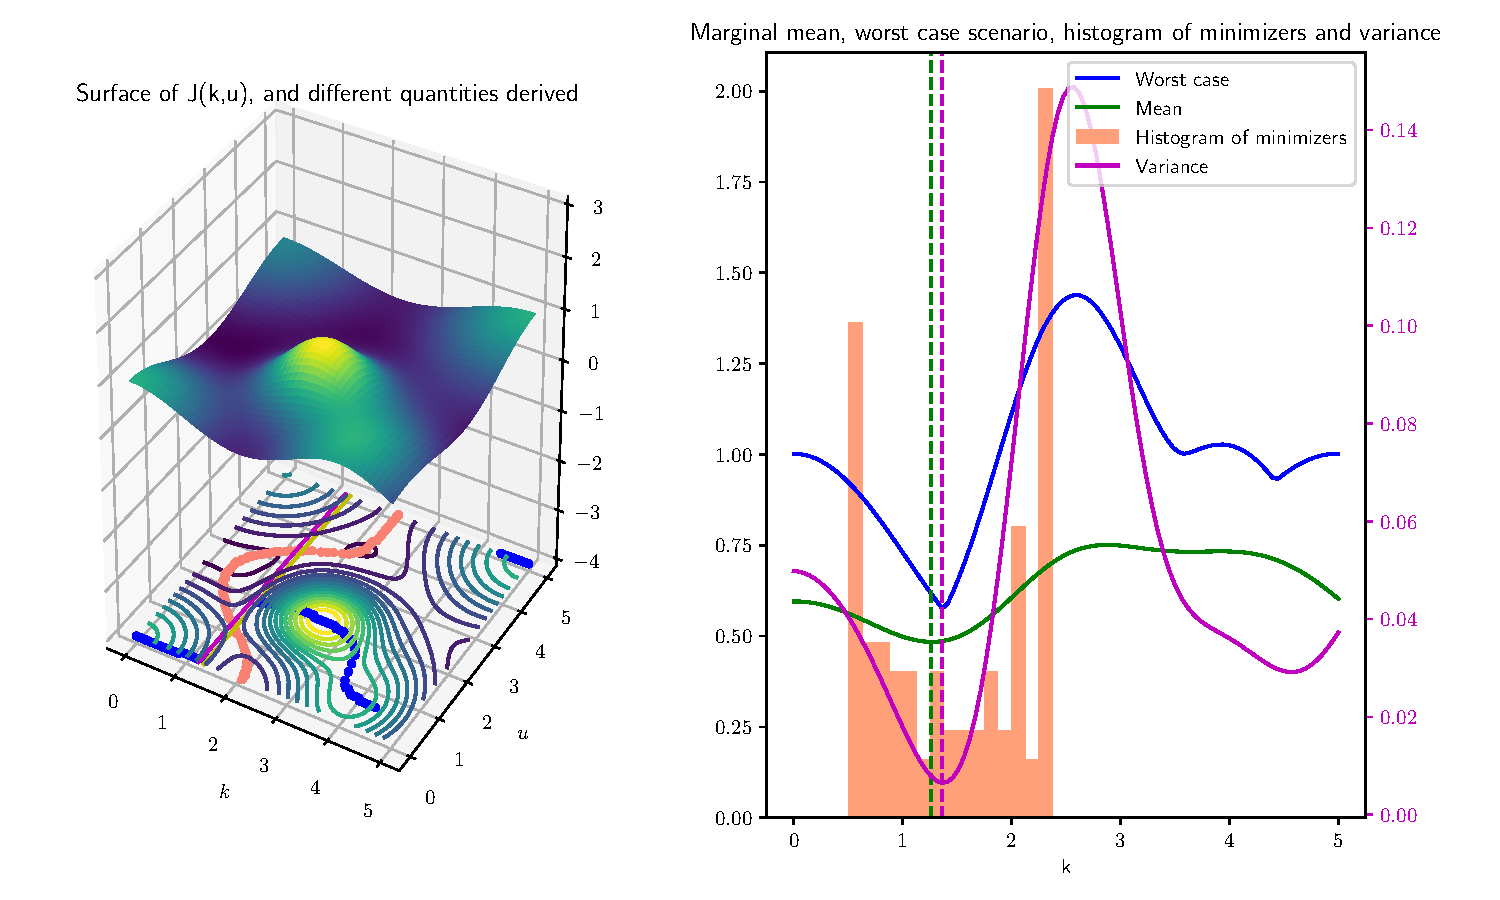
\includegraphics[width = .85\linewidth]{surface_transp_horiz}
    \end{figure}
  \end{block}
\end{column}

\begin{column}{\sepwid}\end{column} % Empty spacer column
\begin{column}{\sndcolwid} % Begin a  column which is two columns wide (column 2)
 


%
  

  
 

\begin{block}{General methods}
  \begin{itemize}\large

  \item Design of Experiment
    \begin{itemize}
    \item Efficient exploration of the input space: LHS, space filling designs
    \end{itemize}
    % \begin{wrapfigure}{r}{.1\linewidth}
    %   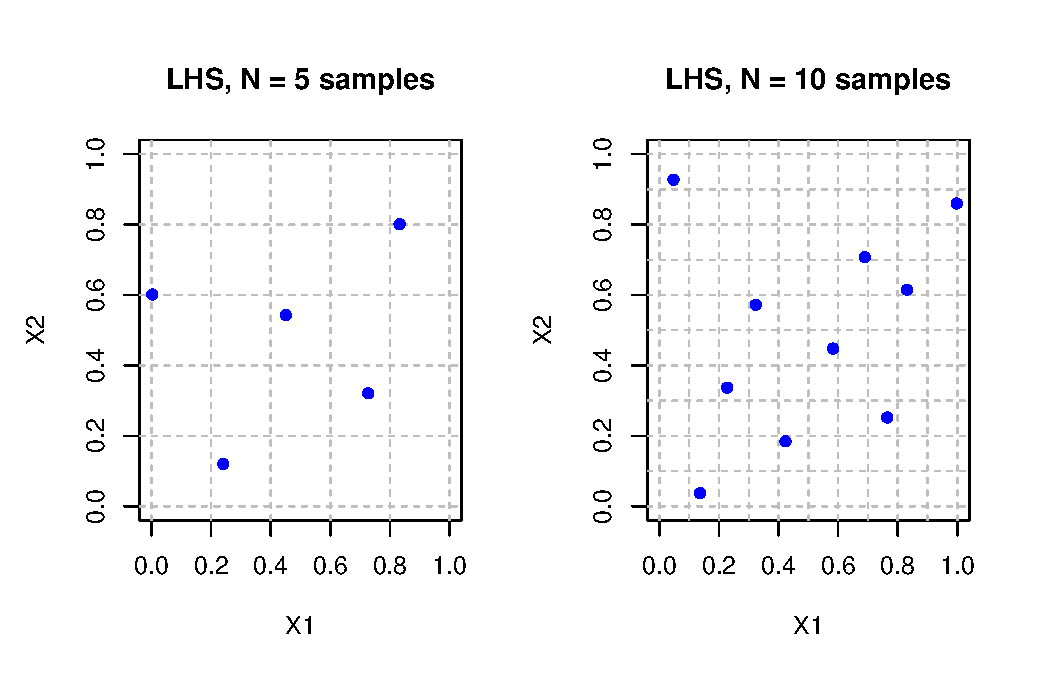
\includegraphics[scale = 1]{LHSsample}
    % \end{wrapfigure}
  \item Statistical/Probabilistic aspects
    \begin{itemize}
    \item Bayesian/Frequentist approach: Markov-chain based methods, study of the posterior distribution
    \item Choice of prior on $\bm{K}$ to take into account specific information on spatial variation of the friction
    \item Marginalization with respect to $\bm{U}$
    \end{itemize}
  \item Surrogate modelling
    \begin{itemize}
    \item Kriging (Gaussian Process Regression)
    \item Polynomial Chaos Expansion
    \end{itemize}
  \item Optimization
    \begin{itemize}
    \item Adjoint method provides the gradient of the cost function $\rightarrow$ Adapt principles of gradient descent on specific objectives
    \item Adaptative sampling: based on surrogate, choose the next point to be evaluated based on a specific criterion: EGO, IAGO and more general \emph{Stepwise Uncertainty Reduction} strategies \nocite{jones_efficient_1998}
    \end{itemize}
  \end{itemize}
\end{block}
% % ----------------------
% ------------------------------------------------------------
\begin{block}{Numerical Results: toy model of Shallow Waters}
  \begin{center}
    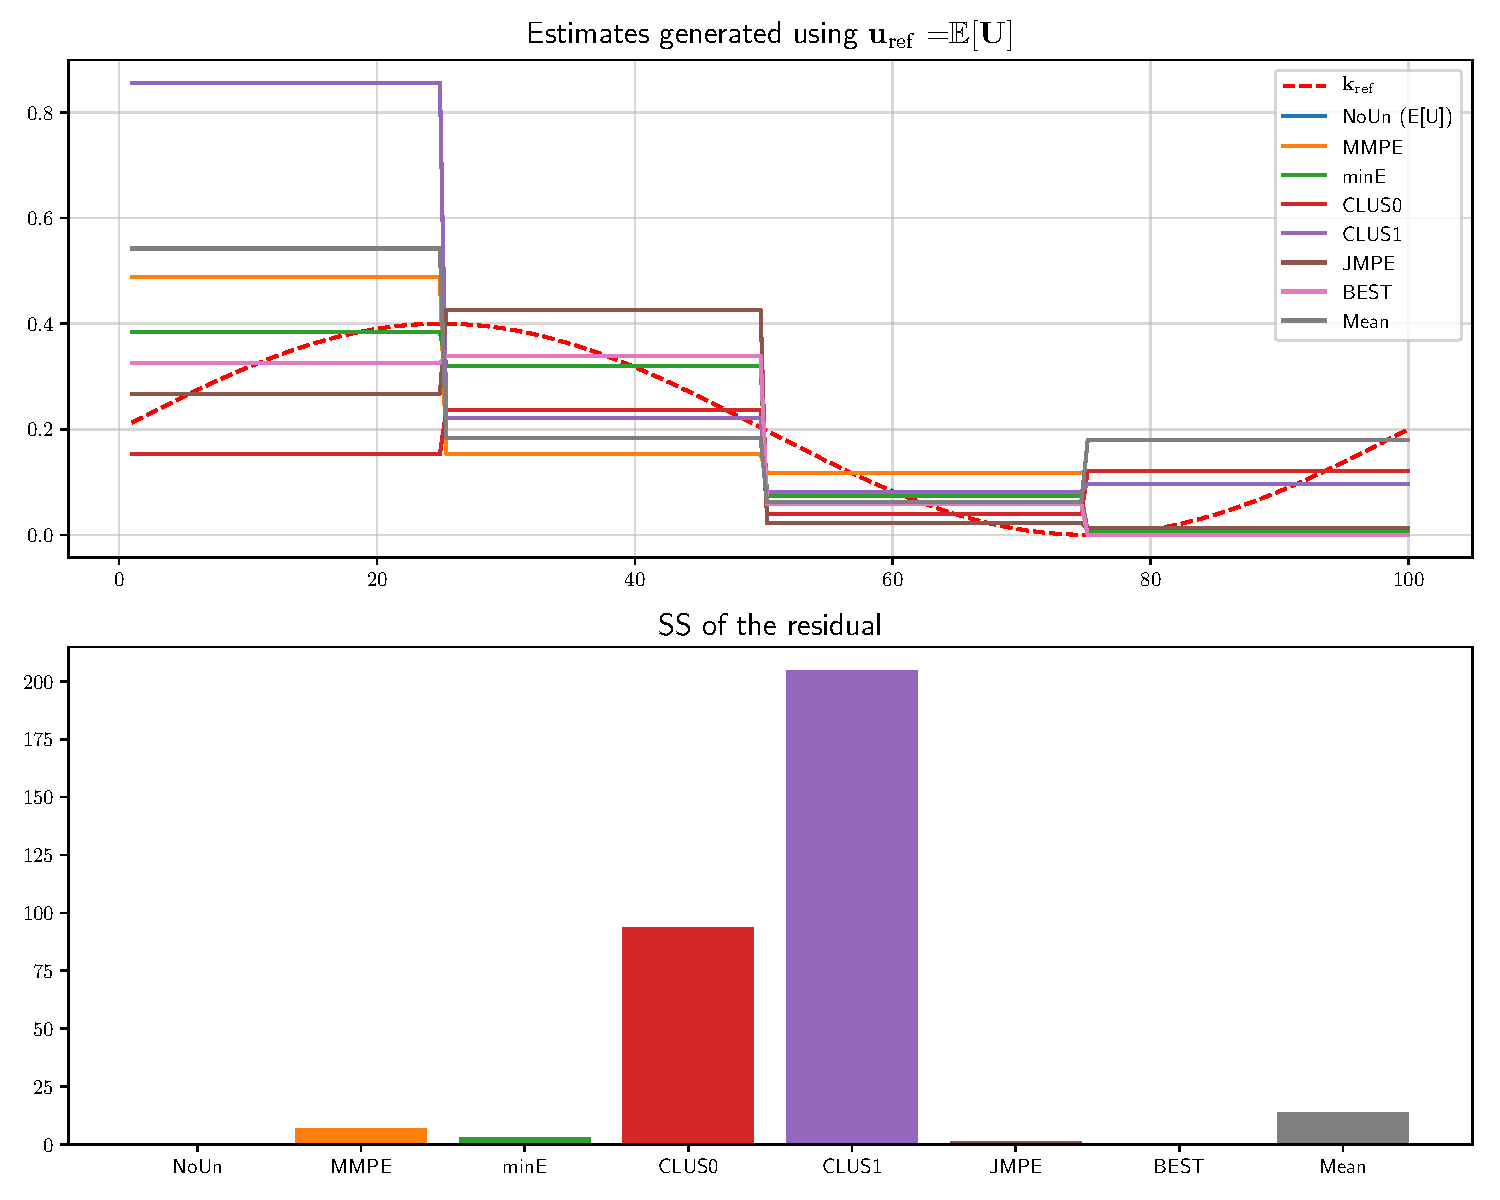
\includegraphics[width = .97\textwidth]{estimate_uref_centered.pdf}
  \end{center}
  \begin{center}
    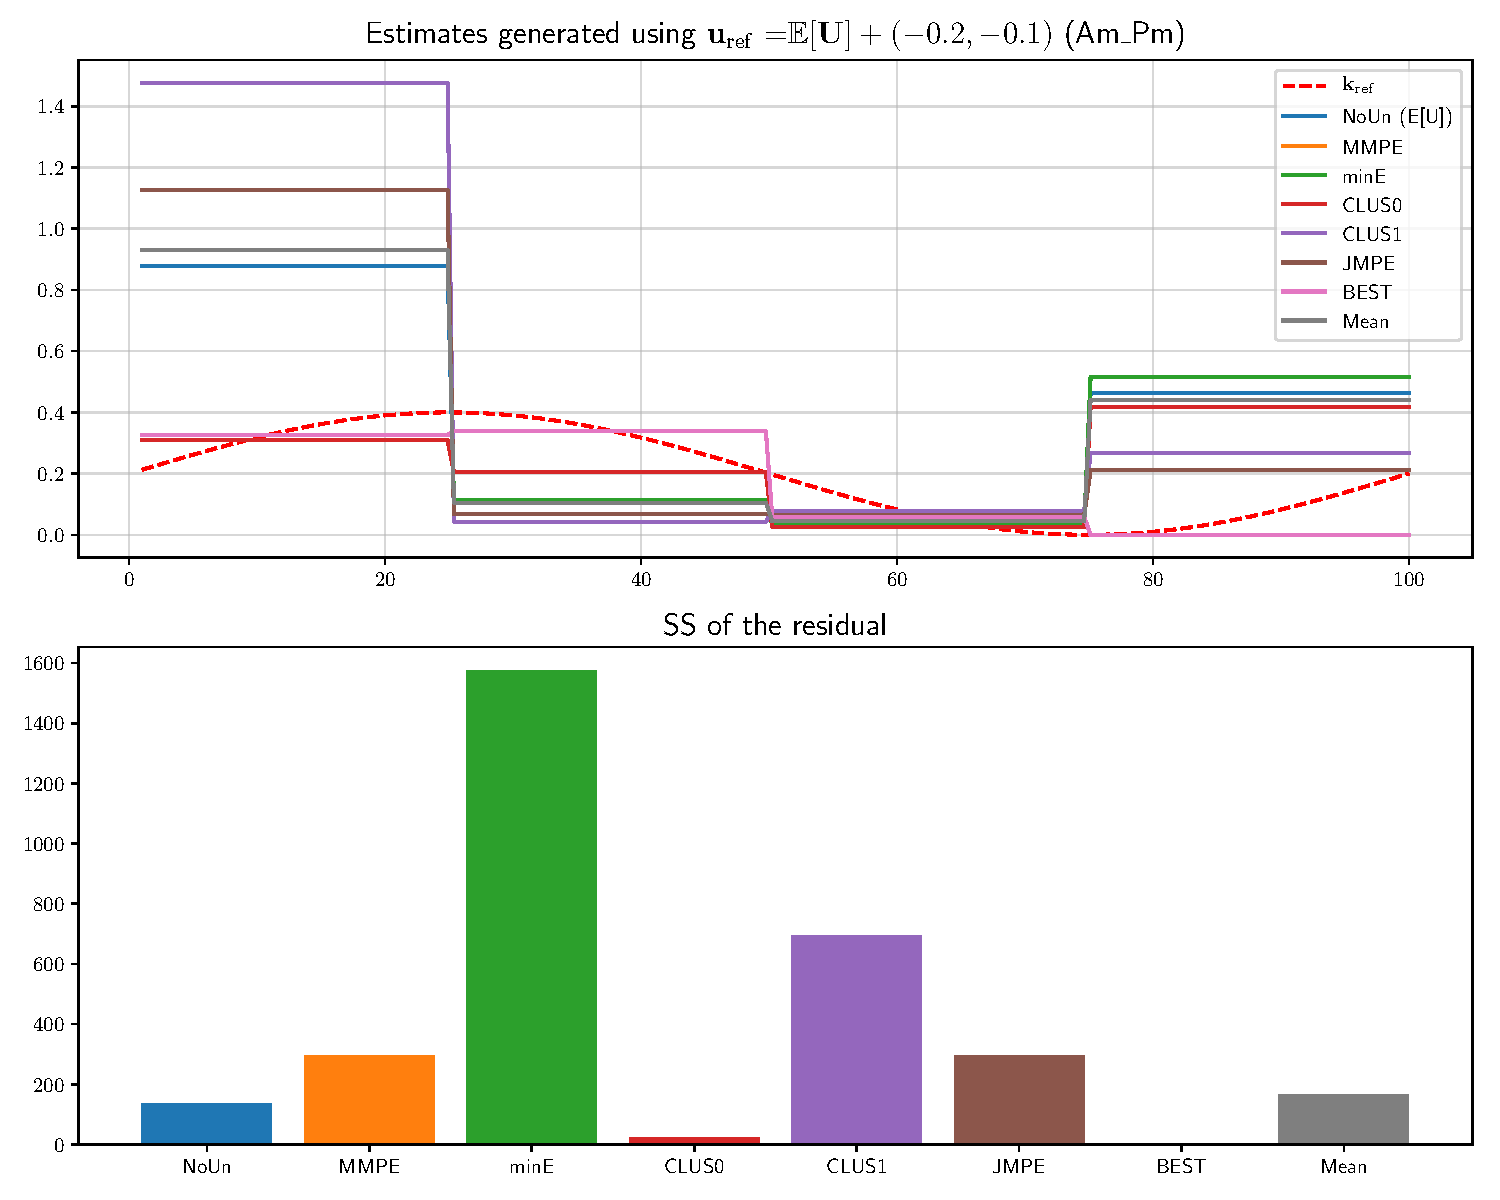
\includegraphics[width = .97\textwidth]{estimate_uref_AmPm.pdf} 
  \end{center}
\end{block}
\vfill
\begin{block}{Conclusion and perspectives}
  \begin{itemize}
  \item Several objectives can be defined, often concurrent
  \item Choice of criterion of robustness is application-dependent
  % \item Use of \alert{Surrogate Models} ?
  \item Scalability of methods in high dimension ? Need to perform \alert{Dimension reduction} on $\mathcal{K}$ and  $\mathcal{U}$
  \end{itemize}
\end{block}

%----------------------------------------------------------------------------------------



\end{column} % End of column 2

\begin{column}{\sepwid}\end{column} % Empty spacer column


% %----------------------------------------------------------------------------------------
% \end{column} % End of the second column

\begin{column}{\leftmar}
\end{column} % Empty spacer column



\end{columns}
% \vspace{2ex}
% \vfill
\begin{columns}

  \begin{column}{\leftmar}
  \end{column} % Empty spacer column
{\scriptsize
  \begin{column}{\centercol}
    \begin{block}{References}
     \vspace{-2ex}
      \begin{multicols}{5}
        \bibliographystyle{unsrt} 
        \bibliography{./bibzotero}
      \end{multicols}
     
      
      % \end{columns}
    \end{block}
  \end{column}
  }
  \begin{column}{\leftmar}
  \end{column} % Empty spacer column
  
\end{columns}
\vfill
\end{frame}
\end{document}

%%% Local Variables:
%%% mode: latex
%%% TeX-master: t
%%% End: